%------------------------
% Resume Template
% Author : Anubhav Singh
% Github : https://github.com/xprilion
% License : MIT
% Original Template: https://www.overleaf.com/latex/templates/resume-template-by-anubhav/dhmkrwtksdgy
%------------------------

\documentclass[letterpaper,10pt]{article}

\usepackage{latexsym}
\usepackage[empty]{fullpage}
\usepackage{titlesec}
\usepackage{marvosym}
\usepackage[usenames,dvipsnames]{color}
\usepackage{verbatim}
\usepackage{enumitem}
\usepackage[pdftex]{hyperref}
\usepackage{fancyhdr}

% For images
\usepackage{graphicx}
\usepackage{caption}
\usepackage{subcaption}

\pagestyle{fancy}
\fancyhf{} % clear all header and footer fields
\fancyfoot{}
\renewcommand{\headrulewidth}{0pt}
\renewcommand{\footrulewidth}{0pt}

% Adjust margins
\addtolength{\oddsidemargin}{-0.530in}
\addtolength{\evensidemargin}{-0.375in}
\addtolength{\textwidth}{1in}
\addtolength{\topmargin}{-.45in}
\addtolength{\textheight}{1in}

\urlstyle{rm}

\raggedbottom
\raggedright
\setlength{\tabcolsep}{0in}

% Sections formatting
\titleformat{\section}{
  \vspace{-10pt}\scshape\raggedright\large
}{}{0em}{}[\color{black}\titlerule \vspace{-6pt}]

%-------------------------
% Custom commands
\newcommand{\resumeItem}[2]{
  \item\small{
    \textbf{#1}{: #2 \vspace{-2pt}}
  }
}

\newcommand{\resumeItemWithoutTitle}[1]{
  \item\small{
    {\vspace{-2pt}}
  }
}

\newcommand{\resumeSubheading}[4]{
  \vspace{-1pt}\item
    \begin{tabular*}{0.97\textwidth}{l@{\extracolsep{\fill}}r}
      \textbf{#1} & #2 \\
      \textit{#3} & \textit{#4} \\
    \end{tabular*}\vspace{-5pt}
}

\newcommand{\educationSubheading}[5]{
  \vspace{-1pt}\item
    \begin{tabular*}{0.97\textwidth}{l@{\extracolsep{\fill}}r}
      \textbf{#1} & #2 \\
      \textit{#3}\textbf{#4} & \textit{#5} \\
    \end{tabular*}\vspace{-5pt}
}


\newcommand{\resumeSubItem}[2]{\resumeItem{#1}{#2}\vspace{-3pt}}

\renewcommand{\labelitemii}{$\circ$}

\newcommand{\resumeSubHeadingListStart}{\begin{itemize}[leftmargin=*]}
\newcommand{\resumeSubHeadingListEnd}{\end{itemize}}
\newcommand{\resumeItemListStart}{\begin{itemize}}
\newcommand{\resumeItemListEnd}{\end{itemize}\vspace{-5pt}}
\newcommand{\qrheader}[1]{
  \begin{center}
    \vspace{0.5cm}
    \textbf{#1}
    % \vspace{-0.5cm}
  \end{center}
}

%-----------------------------
%%%%%%  RESUME STARTS HERE  %%%%%%
\begin{document}

%-----------QR CODES-----------------
\section{Portfolio Quick Access}

  \begin{center}
    \qrheader{CMU Research}
    \begin{minipage}{0.45\textwidth}
        \centering
        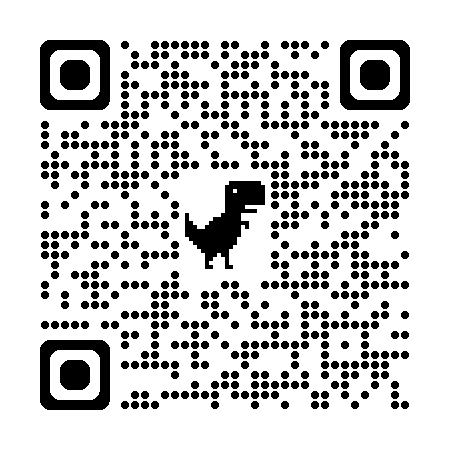
\includegraphics[width=6.5cm, height=6.5cm]{Figures/Zoe.png}
        \captionof{figure}{Zoë Rover}
        \label{fig:image1}
    \end{minipage}
    \hspace{0.05\textwidth}
    \begin{minipage}{0.45\textwidth}
        \centering
        
\includegraphics[width=6.5cm, height=6.5cm]{Figures/HUMRS.png}
        \captionof{figure}{Underwater Snake Robot}
        \label{fig:image2}
    \end{minipage}
    \vspace{0.1cm} % Space between rows
  \end{center}

  \begin{center}
    \qrheader{Finished Projects}
    \begin{minipage}{0.45\textwidth}
        \centering
        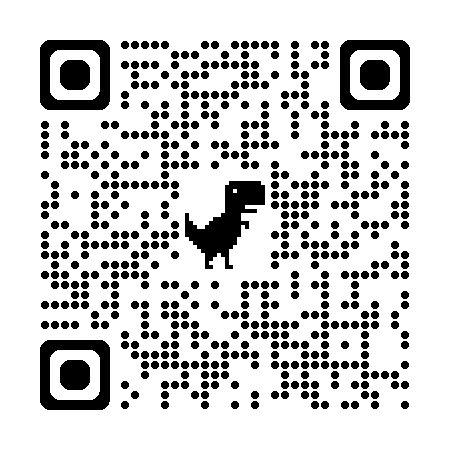
\includegraphics[width=6.5cm, height=6.5cm]{Figures/STM32.png}
        \captionof{figure}{STM32 Elevator Simulator}
        \label{fig:image3}
    \end{minipage}
    \hspace{0.05\textwidth}
    \begin{minipage}{0.45\textwidth}
        \centering
        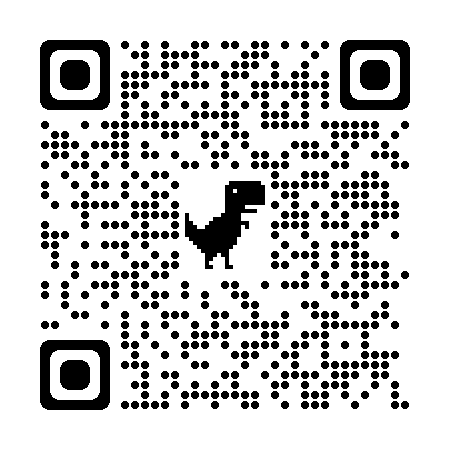
\includegraphics[width=6.5cm, height=6.5cm]{Figures/CustomCane.png}
        \captionof{figure}{Custom Cane}
        \label{fig:image4}
    \end{minipage}
    \vspace{0.1cm} % Space between rows
  \end{center}
  
  \begin{center}
    \qrheader{High School Robotics}
    \begin{minipage}{0.45\textwidth}
        \centering
        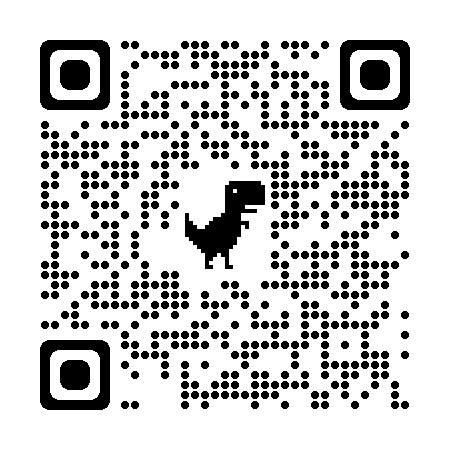
\includegraphics[width=6.5cm, height=6.5cm]{Figures/DEWBOTXVII.png}
        \captionof{figure}{Dewbot XVII}
        \label{fig:image5}
    \end{minipage}
    \hspace{0.05\textwidth}
    \begin{minipage}{0.45\textwidth}
        \centering
        
\includegraphics[width=6.5cm, height=6.5cm]{Figures/VEX.png}
        \captionof{figure}{VEX Robotics}
        \label{fig:image6}
    \end{minipage}
  \end{center}

\end{document}